\documentclass[12pt]{article}
\usepackage{ctex}
\usepackage[english]{babel}
\usepackage{blindtext}
\usepackage{nameref}
\usepackage{fancyhdr}
\usepackage{amsmath,amssymb,amsthm}
\usepackage{graphicx,float}
\usepackage{physics}
\usepackage{pgfplots}
\usepackage[a4paper, total={6in, 9in}]{geometry}

\graphicspath{{../image/}}

\pagestyle{fancy}
\fancyhf{}
\fancyhf[HL]{矩陣附加引導練習}
\fancyhf[CF]{\thepage}

\newcommand{\innerprod}[2]{\langle{#1},{#2}\rangle}
\newcommand{\id}{\mathtt{id}}
\newcommand{\rref}{\mathrm{RREF}}
\newcommand{\adj}{\mathrm{adj}}

\newtheorem{definition}{定義}
\newtheorem*{theorem}{定理}
\newtheorem*{corollary}{衍理}
\newtheorem*{lemma}{引理}
\newtheorem*{proposition}{命題}
\newtheorem*{remark}{小記}
\newtheorem*{claim}{主張}
\newtheorem*{example}{示例}
\newtheorem*{axiom}{公設}
\renewenvironment*{proof}{\textit{證明.}}{\hfill$\qed$}

\newenvironment*{sol}{\par \textbf{解}.}{\hfill$\blacksquare$}

\begin{document}
    此練習在於延伸並引導學習至矩陣對數。
    \begin{enumerate}
        \item 考慮$x=(x_1,x_2,\dots,x_n)\in \mathbf{X}$,且$$y=(y_1,y_2,\dots,y_n)\in \mathbf{X}$$使得下列方程組成立:\begin{align*}
            \begin{cases}
                y_1&=a_{11}x_1+a_{12}x_2+\cdots+a_{1n}x_n\\
                y_2&=a_{21}x_1+a_{22}x_2+\cdots+a_{2n}x_n\\
                &\vdots\\
                y_n&=a_{n1}x_1+a_{n2}x_2+\cdots+a_{nn}x_n
            \end{cases}
        \end{align*}
        \begin{enumerate}
            \item 試以$y=Ax$的形式表以上方程組。
            \item 現知道$$\begin{bmatrix}
                y_{11}&y_{12}&\cdots&y_{1n}\\
                y_{21}&y_{22}&\cdots&y_{2n}\\
                \vdots&\vdots&\ddots&\vdots\\
                y_{n1}&y_{n2}&\cdots&y_{nn}
            \end{bmatrix}=A\begin{bmatrix}
                x_{11}&x_{12}&\cdots&x_{1n}\\
                x_{21}&x_{22}&\cdots&x_{2n}\\
                \vdots&\vdots&\ddots&\vdots\\
                x_{n1}&x_{n2}&\cdots&x_{nn}
            \end{bmatrix}$$,若表$\mathbf{y}_k=\begin{bmatrix}
                y_{1k}\\
                y_{2k}\\
                \vdots\\
                y_{nk}
            \end{bmatrix}$及$\mathbf{x}_k=\begin{bmatrix}
                x_{1k}\\
                x_{2k}\\
                \vdots\\
                x_{nk}
            \end{bmatrix}$,證明$\mathbf{y}_k=A\mathbf{x}_k$。
            \item 由此,描述(b)的方程組的幾何意義。
        \end{enumerate}
        \item 設$A\in\mathbb{M}^{n\times n}$為可對角化矩陣,使得存在可逆矩陣$P$及對角矩陣$D$令$A=P^{-1}DP$成立,並設$f(x):=Ax$,其中$x\in\mathbb{R}^n$。\begin{enumerate}
            \item 試就以下圖像解釋$f$的幾何含義:
            \begin{figure}[H]
                \centering
                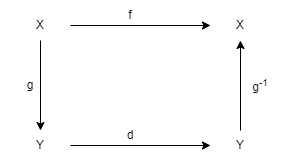
\includegraphics[scale=0.6]{commutative_diagram_diagonalization.png}
            \end{figure}
            其中$g(x):=Px$及$d(x):=Dx$,$X$及$Y$為不同基底的綫性空間。
            \item 證明以下定理:\begin{theorem}
                若$X$及$Y$的維數不同,則不存在可逆矩陣$B$使得$B:X\leftrightarrow Y$。
            \end{theorem}
            提示:\begin{enumerate}
                \item 設$X$的維數為$m$及$Y$的維數為$n$,且$m>n$,以此建立合適的矩陣$B:X\mapsto Y$。
                \item 證明該矩陣$B$不可逆。
                \item 同理當$m<n$時,考慮$B:Y\mapsto X$。
            \end{enumerate}
            \item 由此,討論‘不可被對角化’的幾何含義。
        \end{enumerate}
        \item \begin{enumerate}
            \item 利用基本原理,證明以下矩陣導數法則:\begin{enumerate}
                \item $\dfrac{d}{dt}A=0$;
                \item $\dfrac{d}{dt}At^n=nAt^{n-1}$;
                \item $\dfrac{d}{dt}e^{At}=Ae^{At}=e^{At}A$;
            \end{enumerate}
            \item 證明以下定律對矩陣導數適用:\begin{enumerate}
                \item 乘積法則;
                \item 鎖鏈法則。
            \end{enumerate}
            \item 由此,求導$\dfrac{d}{dt}t^{A}$。
        \end{enumerate}
        \item 已知矩陣的指數法$e^{A}$,現求矩陣的對數法。記矩陣的對數函數為$\log{X}$使得$e^{\log{X}}=e^{\log{X}}=X$。\begin{enumerate}
            \item 證明$|e^A|=e^{|A|}$。由此證明若$\log{X}$存在,則$|X|> 0$。
            \item 證明若$X$可對角化成$P^{-1}DP$,則$\log{X}=P^{-1}(\log{D})P$。
            \item 求導$\dfrac{d}{dt}\log{(Xt)}$。
        \end{enumerate}
    \end{enumerate}
\end{document}